\section{Concept}
In this section a concept of a mobile \enquote{\gls{see}} version will be presented. 
Therefore, a prototype will be created to point out the features that a mobile version of \enquote{\gls{see}} requires.

Prototypes are a common way to express the needs of a system. 
It is a low-cost way of planning an implementation, that can highlight challenges regarding constraints of a system early on.

Even though a prototype will never be able to show every aspect and need of a complex system, it should still help to answering questions like: 
How should the system feel? How should it be implemented and what are the key features? \cite{houde1997prototypes} 

\enquote{\gls{see}} is meant to be used by multiple platforms such as desktop devices, mobile devices and virtual reality devices.
Each device has different interaction constrains. 
While a desktop user will control the player with mouse and keyboard a mobile user will interact with virtual joysticks on a touchscreen.
Selecting nodes of a \enquote{\gls{city}} will be done by clicking it with a mouse on desktop devices, while a mobile device will require a touch input.

\subsection{Interface}

In the following a paper prototype will be presented that marks out a concept for the mobile interface.
Since the field of mobile development is quite young there few guidelines regarding the design of mobile device interfaces.
A guideline that is widely accepted is problematic to find. \cite{renaud2017demarcating}, \cite{punchoojit2017usability}

Major differences to desktop environments are the screen size, forms of input and input feedback.
To assure as much space is used for the actual interaction of the app the menu should just take as much space as needed.
As a study has found out, a size of at least 8*8 mm is needed to reduce error rates selecting the right button. \cite{conradi2015optimal}
TODO WEITER AUSFÜHREN
SHORTCUTS WIE STRG Z NICHT MÖGLICH
 \cite{adipat2005interface} 

Moving the player will be handled with virtual joysticks as seen in figure \ref{fig:joystick}.
The left joystick will move the player through the virtual room and the right will move the camera angle or in other word the direction the player looks at.
The joysticks are placed in the left and right corner and should just take as much space as needed to be handled comfortably.
This way the player is able to navigate through the virtual room with his/her thumps while still having enough space to work on the \enquote{\gls{city}}.

\begin{figure}[htb]
    \centering
    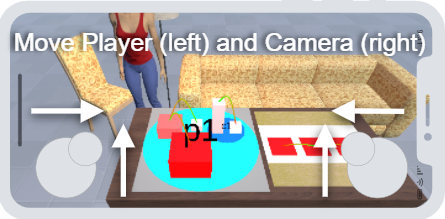
\includegraphics[width=1\textwidth]{Concept/img/joystick.png}
    \caption{Joysticks for moving in \enquote{\gls{see}}}\label{fig:joystick}
\end{figure}

The menu on the top left side seen in figure \ref{fig:quickbar} will be called "quickbar" further on. 
The quickbar can be minimized to safe screen space when not needed. 
The quickbar is designed to offer more general functions that are needed in various situations.
Because there are no shortcuts on mobile devices each function has to have a button to be activated.

The functions are redo and undo which will do an action undone again or revert an action.
Then there is a camera lock that will lock the players perspective to a certain \enquote{\gls{city}} so that the player can only move around the selected city and move closer or further away from it.
The next function is to rerotate a \enquote{\gls{city}}.
That means the \enquote{\gls{city}} that was last rotated will be set back to its initial state of rotation.
Last but not least there will be a button for recentering the city, which will work quite similar to the rerotate button and center the last moved \enquote{\gls{city}}.
The button on the right can be used to collapse or expand the quickbar.
\begin{figure}[htb]
    \centering
    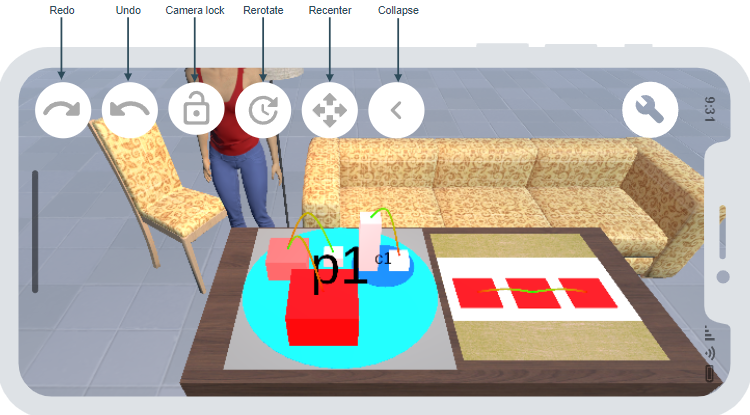
\includegraphics[width=1\textwidth]{Concept/img/quickbar.png}
    \caption{Quickbar for various interactions in \enquote{\gls{see}}}\label{fig:quickbar}
\end{figure}

On the top right side another menu will be placed that contains different interaction modes.
\begin{figure}[htb]
    \centering
    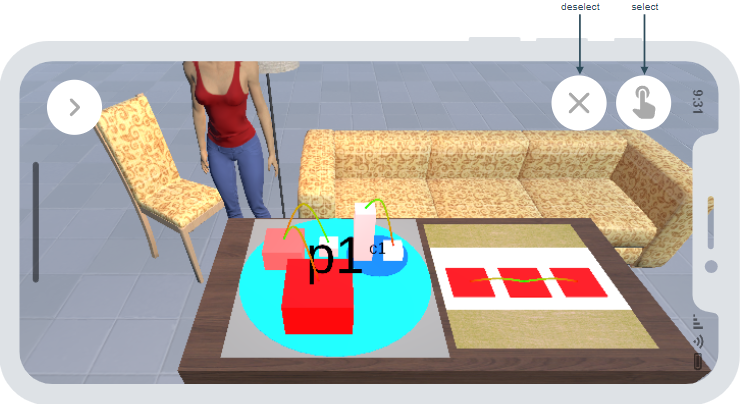
\includegraphics[width=1\textwidth]{Concept/img/menu1.png}
    \caption{Selection mode in \enquote{\gls{see}}}\label{fig:select}
\end{figure}

\begin{figure}[htb]
    \centering
    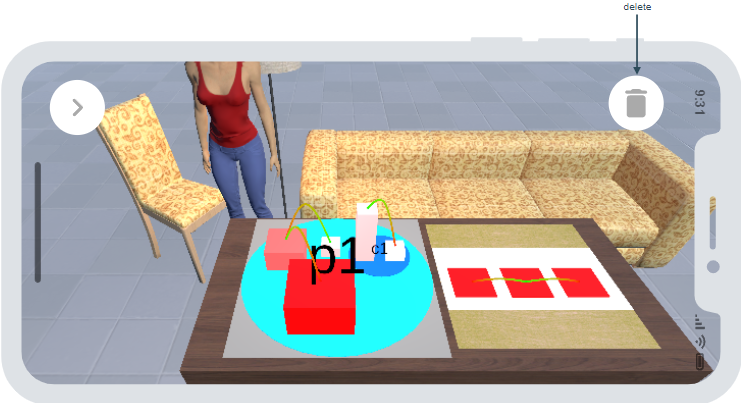
\includegraphics[width=1\textwidth]{Concept/img/menu2.png}
    \caption{Delete mode in \enquote{\gls{see}}}\label{fig:delete}
\end{figure}

\begin{figure}[htb]
    \centering
    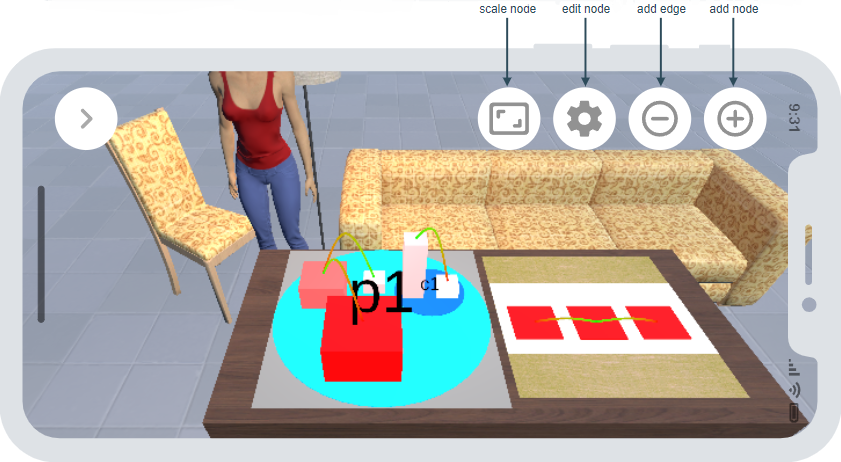
\includegraphics[width=1\textwidth]{Concept/img/menu3.png}
    \caption{Node interactions in \enquote{\gls{see}}}\label{fig:nodes}
\end{figure}

\begin{figure}[htb]
    \centering
    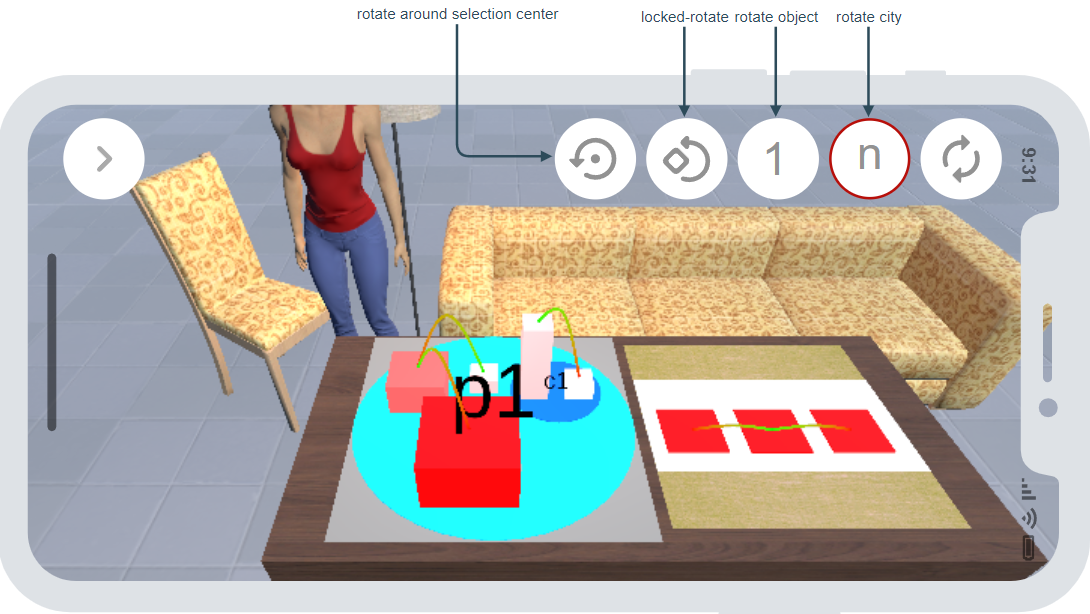
\includegraphics[width=1\textwidth]{Concept/img/menu4.png}
    \caption{Rotation mode in \enquote{\gls{see}}}\label{fig:rotate}
\end{figure}

\begin{figure}[htb]
    \centering
    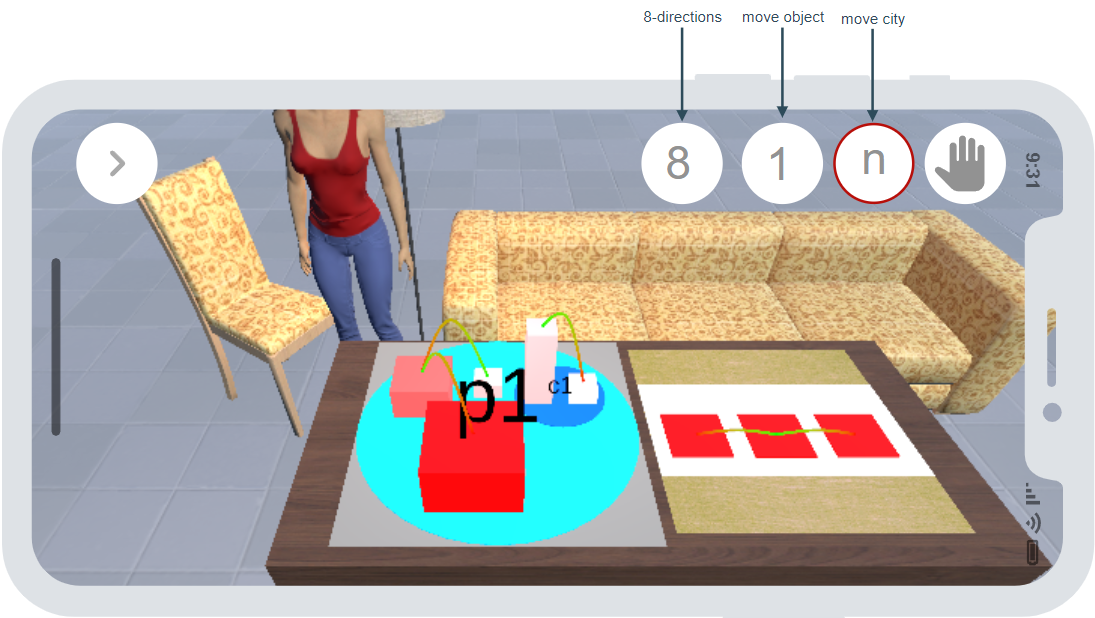
\includegraphics[width=1\textwidth]{Concept/img/menu5.png}
    \caption{Movement mode in \enquote{\gls{see}}}\label{fig:move}
\end{figure}

\subsection{Interaction}
...
\subsection{Requirements}
In the following a list of requirements will be given, which will specify in detail what the implementation of a mobile version has to take care of.
The list will be referred to multiple times in the upcoming realization part in chapter \ref{section:implementation}.
Requirements are essential for the planning phase as they give a good fundamental structure for the developer to rely on. \cite{Robertson2012,Stevens2005}